\documentclass[11pt]{article} \setlength{\oddsidemargin}{0in}
\setlength{\evensidemargin}{0in} \setlength{\textwidth}{6.5in}
\setlength{\parindent}{0in} \setlength{\textwidth}{16cm}
\setlength{\topmargin}{1in} \addtolength{\topmargin}{-1.5in}
\setlength{\textheight}{23cm} \setlength{\parskip}{0.75cm}

\usepackage {fancyvrb}
\newenvironment{qv}
{\quote\Verbatim}{\endVerbatim\endquote}


\usepackage[dvipsnames]{xcolor}


% Brackets
\usepackage{mathtools, tikz-qtree} \DeclarePairedDelimiter\ceil{\lceil}{\rceil}
\DeclarePairedDelimiter\floor{\lfloor}{\rfloor}

% Tikz settings
\usepackage{tikz} \usetikzlibrary{trees} \usetikzlibrary {positioning}
\definecolor {mypurple}{cmyk}{0.6,0.4,0.1,0} \definecolor
{myred}{cmyk}{0,0.3,0.3,0} \usetikzlibrary{fit,shapes.misc}

\usetikzlibrary{trees}
\tikzset{every tree node/.style={minimum width=2em,draw,rectangle},
         blank/.style={draw=none},
         edge from parent/.style=
         {draw,edge from parent path={(\tikzparentnode) -- (\tikzchildnode)}},
         level distance=1.5cm}

% Typesetting options
\usepackage{fancyvrb} \usepackage{amsmath,amsfonts,amssymb}
\usepackage [english]{babel} \usepackage [autostyle, english =
american]{csquotes} \usepackage[none]{hyphenat} \usepackage{url}

% Graph
\usepackage{tikz}
\tikzstyle{level 3} = [level distance = 4cm , sibling distance = .5cm]
\tikzstyle{level 2} = [level distance = 3cm , sibling distance = .5cm]
\tikzstyle{level 1} = [level distance = 3cm , sibling distance = .5cm]

\begin{document}

\noindent CSCI 3104 Spring 2018 \hfill Problem Set 4\\
Erika Bailon (09/28)

\hrulefill

{\fontfamily{cmr}\selectfont

  % ******************* PROBLEM 1 *********************
  \section*{Problem 1}

  \textit{(10 pts) Suppose that we modify the \texttt{Partition}
    algorithm in QuickSort in such a way that on on every third level
    of the recursion tree it chooses the worst possible pivot, and on
    all other levels of the recursion tree \texttt{Partition} chooses
    the best possible pivot.  Write down a recurrence relation for
    this version of QuickSort and give its asymptotic solution. Then,
    give a verbal explanation of how this \texttt{Partition} algorithm
    changes the running time of QuickSort.}

To find the recurrance relationship we look at the recurrence on each level:\\
The 1$^{st}$ level has the recurrence $T_1(n) = 2 \cdot T_2(\frac{n}{2}) + \Theta(n)$\\
The 2$^{nd}$ level has the recurrence $T_2(n) = 2 \cdot T_3(\frac{n}{2}) + \Theta (n)$\\
The 3$^{rd}$ level has the recurrence $T_3 (n)= T_1(n-1) + \Theta (n)$\\
Unrolling (or substituting) we get: \\
$T_2(n) = 2 \cdot T_1(\frac{n-1}{2}) + \frac{1}{2}\Theta(n) + \Theta(n) \rightarrow \cdot T_1(\frac{n-1}{2}) + \frac{3}{2}\Theta(n)$\\
$T_1(n) = 2 \cdot 2 \cdot T_1(\frac{n-1}{4}) + \frac{3}{4}\Theta(n) + \Theta(n) \rightarrow 4 \cdot T_1(\frac{n-1}{4}) + \frac{7}{4}\Theta(n)$ \\
Since $T_1(\frac{n-1}{4}) \leq T_1(\frac{n}{4})$ and since $\frac{7}{4}\Theta(n) = \frac{7}{4} \cdot C(n) = \Theta(n)$\\
$\Rightarrow$ we get then that $\mathbf{T (n)= 4 \cdot T(\frac{n}{4}) + \Theta(n)}$. \\
Analyzing this recurrence with the Master Theorem we obtain that: \\
$\mathbf{T(n) = \Theta(n lg (n))}$ \\\\
This $Partition$ algorithm changes the running time every 3 levels. As I explained before with the recurrence of each level, we have the best case scenario from level $1$ to level $2$, and another best case scenario from level $2$ to level $3$. The best case scenario is when the pivot is chosen in the partition $\frac {n}{2}$, which is the element in the middle of the array, but then when is running level number $3$ it choses the worst pivot, which will be $n-1$, this affects the running time making the process longer, more time to sort the array. 

\newpage

  % ******************* PROBLEM 2 *********************
  \section*{Problem 2}

  \textit{(10 pts) Mr. Ollivander, of Ollivanders wand shop, has hired
    you as his assistant, to find the most powerful wand in the
    store. You are given a magical scale which ``weighs'' wands by how
    powerful they are (the scale dips lower for the wand which is more
    powerful). You are given n wands $W_1, \dots ,W_n$, each having
    distinct levels of power (no two are exactly equal).}

  \begin{enumerate}
  \item[(a)]{\textit{Consider the following algorithm to find the most %*******a******%
        powerful wand:}}
    \begin{enumerate}
    \item[i.] \textit{Divide the n wands into $\frac{n}{2}$ pairs of
        wands.}
    \item[ii.] \textit{Compare each wand with its pair, and retain the
        more powerful of the two.}
    \item[iii.] \textit{Repeat this process until just one wand
        remains.}
    \end{enumerate}

    \textit{Illustrate the comparisons that the algorithm will do for
      the following n = 8 input:}

    $$
    W_1:\frac{3}{2},\; W_2:\frac{5}{2},\; W_3:\frac{1}{2},\; W_4:1,\;
    W_5:2,\; W_6:\frac{5}{4},\; W_7:\frac{1}{4}\;, W_8:\frac{9}{4}
    $$
    \\

To illustrate the comparisons we can use a repechage, is like a chart of elimination where we have brackets of the wands being compared to see which one "wins" and goes to the next level/bracket to compete with the ones that won on the other brackets. I will try to illustrate here:  *** RED is losers ***GREEN is winers - on each level in the bracket the winner goes to the next level\\\\

\begin{tikzpicture}[grow = left, sloped]
  \Tree
  [. {\color{Green}\textbf{W2: 5/2}}
  	[. {\color{Green}\textbf{W2: 5/2}}
      [. {\color{Green}\textbf{W2: 5/2}}
        [.{\color{red} \textbf{W1: 3/2}}
        ]
        [. {\color{Green}\textbf{W2: 5/2}}
        ]
      ]
      [. {\color{red}\textbf{W4: 1}}
        [.{\color{red}\textbf{W3: 1/2}}
        ]
        [. {\color{Green}\textbf{W4: 1}}
        ]
      ]
    ]
    [. {\color{red} \textbf{W8: 9/4}}
      [.  {\color{red}\textbf{W5: 2}}
       [. {\color{Green}\textbf{W5: 2}}
      	]	
        [. {\color{red}\textbf{W6: 5/4}}
      	]
      ]	
      [. {\color{Green}\textbf{W8: 9/4}}
        [. {\color{red}\textbf{W7: 1/4}}
        ]
      	[. {\color{Green}\textbf{W8: 9/4}}
      	]
      ]
    ]
  ]
  \end{tikzpicture}\\
    
  
  \item[(b)]{\textit{Show that for n wands, the algorithm (2a) uses at  %*******b******%
        most n comparisons.}}
    \\\\
    This algorithm is dividing the wands $\frac{n}{2}$ and keeps repeating the process. Therefore we have a recurrence as we have been seen with algorithms that do this type of partition, that fo this is: $T(n) = T(\frac{n}{2}) + \Theta(n)$. Having this we know that the time complexity, or number of comparisons is going to make is equal to: $\Theta(nlg(n))$. \\We know that in case the algorithms does $n$ comparisons it would be $\Theta(n)$. But we know that $\Theta(nlg(n)) \leq \Theta(n)$.  Therefore, we know that is going to take at most  $n$ comparison. \\\\
    (Another way of knowing we will have at most n comparisons is because as we see in the example we first have $\frac{n}{2}$ comparisons. After that we have $\frac{n}{4}$ comparisons then we have  $\frac{n}{8}$ ... if we keep going we see the pattern of the sum that converges to $1$. Which is a constant, and from there we obtain $\Theta(n)$ . Which means again that in the worst case scenario there will be $n$ comparisons.)\\
   
 
  \item[(c)]{\textit{Describe an algorithm that uses the results of (2a).  %*******c******%
        to find the second most powerful wand, using at most $log_2 n$
        additional comparisons. There is no need for pseudocode; just
        write out the steps of the algorithm like we have written in
        (2a). Hint: if you follow sports, especially wrestling, read
        about the \textbf{repechage}.}}
    \\\\
    \textbf{i}. Once you start the main tournament, you take all the losers from the main tournament and put them in a new bracket to start a new competition.\\
    \textbf{ii}. Then you divide the loser wands into pairs of wands to be compared. (If we have an odd number of loser wands, we add the last odd wand to the tournament on the second round. Every wand needs to be compared.)\\
    \textbf{iii}. Repeat this process until we compare the last pair of wands and obtain a single winer! This will be the $second$ most powerful wand.\\\\
    This algorithms will work using at most $log_2n$ because inside of the loop we have going on, we are saving the losers in an array that will be divided to be compared. Comparisons are constant time and we keep dividing the array so worst case would be $log_2n$.
    
  \newpage
  
  \item[(d)]{\textit{Show the additional comparisons that your algorithm.   %*******d******%
        in (2c) will perform for the input given in (2a).}}
    \\\\
    *** RED is losers ***GREEN is winers - on each level in the bracket the winer goes to the next level\\\\
    
    \begin{tikzpicture}[grow = left, sloped]
  \Tree
  [. {\color{Green}\textbf{W8: 9/4}}
  	[. {\color{red}\textbf{W1: 3/2}}
      [. {\color{Green}\textbf{W1: 3/2}}
        [. {\color{Green}\textbf{W1: 3/2}}
        ]
        [. {\color{red}\textbf{W3: 1/2}}
        ]
      ]
      [. {\color{red}\textbf{W6: 5/4}}
        [. {\color{Green}\textbf{W6: 5/4}}
        ]
        [. {\color{red}\textbf{W7: 1/4}}
        ]
      ]
    ]
    [. {\color{Green}\textbf{W8: 9/4}}
      [. {\color{red}\textbf{W5: 2}}
       	[. {\color{red}\textbf{W4: 1}}
      	]	
        [. {\color{Green}\textbf{W5: 2}}
      	]
      ]	
      [. {\color{Green}\textbf{W8: 9/4}}
      ]
    ]
  ]
  \end{tikzpicture}\\

  \end{enumerate}

  \newpage

  % ******************* PROBLEM 3 *********************
  \section*{Problem 3}

  \textit{(20 pts) For obtuse historical reasons, Prof. Dumbledore asks
    his students to line up in ascending order by height in a very tight
    room with little extra space. Similar to Alex the African Grey
    parrot (look it up!), the students, being bored, decided to play a
    little trick on Prof. Dumbledore. They lined up in order by height --
    almost. They made sure that each person was no more than k positions
    away from where they were supposed to be (in ascending order), but
    this allowed them to significantly mess up the precise
    ordering. Here is an example of an array with this property when
    $k = 2$:}



  \begin{tikzpicture}
    \node[] (A0) at (0,4) {A[0]}; \node[] (A1) at (2,4) {A[1]}; \node[]
    (A2) at (4,4) {A[2]}; \node[] (A3) at (6,4) {A[3]}; \node[] (A4) at
    (8,4) {A[4]}; \node[] (A5) at (10,4) {A[5]};

    \node[] (B1) at (0,2) {1}; \node[] (B4) at (2,2) {4}; \node[] (B2)
    at (4,2) {2}; \node[] (B3) at (6,2) {3}; \node[] (B15) at (8,2)
    {15}; \node[] (B5) at (10,2) {5};

    \node[] (C1) at (0,0) {1}; \node[] (C2) at (2,0) {2}; \node[] (C3)
    at (4,0) {3}; \node[] (C4) at (6,0) {4}; \node[] (C5) at (8,0) {5};
    \node[] (C15) at (10,0) {15};

    \draw[->] (B1) -- (C1); \draw[->] (B2) -- (C2); \draw[->] (B3) -- (C3);
    \draw[->] (B4) -- (C4); \draw[->] (B5) -- (C5); \draw[->] (B15) --
    (C15);


  \end{tikzpicture}

  \begin{enumerate}
  \item[(a)]{\textit{Write down pseudocode for an algorithm that would	 %*******a******%
        sort such an array in place--so it fits in the tight room--in time
        $\mathcal{O}(n k \log k)$. Your algorithm can use a function
        $sort(A, l, r)$ that sorts the subarray $A[l],\dots,A[r]$ in
        place in $\mathcal{O}((r-l) \log(r-l))$ steps (assume $r>l$)
        steps (assuming $r > l$).}}
    
    \begin{verbatim}
sorting_nKlogK(A,k):
for (i = 0 to length(A) - k)
{
     sort(A, i , i+k-1)
}
      
\end{verbatim}
    The algorithm will run in  $\mathcal{O}(n k \log k)$ because we have the $for loop$ that is $n$. And then we have the $sort$ function which is ($k \log k$). Therefore we get  $\mathcal{O}(n k \log k)$.\\
  
    
  \item[(b)]{\textit{Suppose you are given to an auxiliary room which.   %*******b******%
        can fit k + 1 students. Modify your previous algorithm to sort
        the given array in time $\mathcal{O}(nk)$.}}
    \\\\
    "I don't know"
    \\
    \newpage
  \item[(c)]{\textit{With the same extra room as in the previous part,    %*******c******%
        modify heap sort using a binary min heap of size $k + 1$ to sort
        the given array in time $\mathcal{O}(n \log k)$.}}
    
     \begin{verbatim}
sortingS(A,k):
for (i = 1 to  k)
{
     B.adding(A[i]).     //We are adding all the element up to k, from A to B.     
}
for (i = 1 to n-k)
{
     A[i] = get_min(B)
     if (i <= n-k+1)
         B.adding(A[i+k])
}
      
\end{verbatim}
  The running time of this algorithm is:
  For the first loop we have $k \log k$ and for the second loop we have $2 \log k$. This gives us a running time of $k \log k + n(2 \log k)$. \\
  However $k \log k \leq n(2 \log k)$ . Also, 2 is a constant so we obtain $\mathcal{O} (n \log k)$. 
  
  \item[(d)]{\textit{(5 pts extra credit) Include the correct story.   %*******d******%
        about Alex, with proper citation. If you wish, you may copy this
        story verbatim, but must indicate clearly that you have done so
        and, of course, still cite your source.}}
     \begin{verbatim}
 The real story about why Alex:
"Alex was an African parrot born in 1976. He became famous for 
being the subject of a psychological experiment at three universities -
University of Arizona, Harvard and Brandeis University.
His uniqueness not only regarded his ability to learn names of individual 
objects but also identify the objects and their colors regardless
of their shape."  - SOURCE 
https://www.thevintagenews.com/2016/11/27/alex-the-
parrot-is-the-only-non-human-to-ask-the-existential-
question-what-color-am-i-2/ 

* I think that the point about the story of Alex in here is why the 
students made a trick to Prof. Dumbledore. The thing was that 
probably, just as Pepperberg has done it with Alex, the 
students of Prof. Dumbledore had been asked for the same 
task over and over again. Therefore they got bored and decided 
to do something different with the task. The task was not 
challenging for the students anymore, just like the same 
questions for Alex was not fun or challenging anymore. 

Alex and the students wanted something different, out of what 
they had been doing for more than one time now. 
I found what happened and how they knew Alex was a living 
entity that could also get bored of the same activities:  "Once, 
Alex was given several different colored blocks (two red, three 
blue, and four green?similar to the picture above). Pepperberg asked 
him, "What color three?" expecting him to say blue. However, as 
Alex had been asked this question before, he seemed to have 
become bored. He answered "five!" This kept occurring until 
Pepperberg said "Fine, what color five?" Alex replied "none". 
This was said to suggest that parrots, like children, get bored. 
Sometimes, Alex answered the questions incorrectly, despite 
knowing the correct answer."  - SOURCE 
https://en.wikipedia.org/wiki/Alex_(parrot) 
   \end{verbatim}

  \end{enumerate}

  \newpage
  % ******************* PROBLEM 4 *********************
  \section*{Problem 4}

  \textit{(20 pts) Consider the following strategy for choosing a pivot
    element for the Partition subroutine of QuickSort, applied to an
    array A.}

  \begin{itemize}
  \item \textit{Let n be the number of elements of the array A}.
  \item \textit{If $n \le 24$, perform an Insertion Sort of A and
      return.}.
  \item \textit{Otherwise:}
    \begin{itemize}
    \item \textit{Choose $ 2 \lfloor n^{1/3} \rfloor $ elements at random from n;
        let S be the new list with the chosen elements.}
    \item \textit{Sort the list S using Insertion Sort and use the
        median m of S as a pivot element.}
    \item \textit{Partition using m as a pivot.}
    \item \textit{Carry out QuickSort recursively on the two parts.}
    \end{itemize}
  \end{itemize}

  \begin{enumerate}
  \item[(a)] \textit{How much time does it take to sort S and     %*******a******%nd its
      median? Give a $\Theta$ bound.}
    \\\\
   We know that $insertionSort$ and $quicksort$ have asymptotically the same worst case scenario which is $\Theta ( n^{2} )$.\\
   In this algorithm we are taking $2n^{\frac{1}{3}}$ elements. Therefore the running time of this algorithm is $\Theta(2n^{\frac{1}{3}})^2$, which is $\Theta \mathbf{4 n^{\frac{2}{3}}}$. 
   For the $\Theta$ bound we have $\Theta(4 n^{\frac{2}{3}})$ because 4 is a constant we have $4 \Theta(n^{\frac{2}{3}}) \rightarrow \mathbf{ \Theta(n^{\frac{2}{3}})}$.
   
  \item[(b)] \textit{If the element m obtained as the median of S is.   %*******b******%
      used as the pivot, what can we say about the sizes of the two
      partitions of the array A?}
    \\\\
    IF the element $m$ obtained as the median of S is used as the pivot to make the partition, then by definition of the median we can see that t $m =\frac {2n^{\frac{1}{3}}}{2}$ and therefore we obtain that $m = n^{\frac{1}{3}}$. Therefore the size of our \textbf{left} array will be $\mathbf{n^{\frac{1}{3}}}$ and the size of the \textbf{right} array will be $\mathbf{n - n^{\frac{1}{3}}}$.
    \\
  \item[(c)] \textit{Write a recurrence relation for the worst case.   %*******c******%
      running time of QuickSort with this pivoting strategy.}
    \\\\
    The recurrence relation we obtain is: $T(n) \leq T(n - 2n^{\frac{1}{3}}) + T(2n^{\frac{1}{3}}) + \Theta(n) + \Theta(n^{\frac{1}{3}}) \rightarrow T(n - 2n^{\frac{1}{3}}) + T(2n^{\frac{1}{3}}) + \Theta(n) \rightarrow T(2n^{\frac{1}{3}}) + \Theta(n)$ (because $T(n - 2n^{\frac{1}{3}}) \leq T(2n^{\frac{1}{3}})$ ) $\Rightarrow  \mathbf{\Theta(n)}$. \\
     
  \end{enumerate}

  \newpage
  % ******************* PROBLEM 5 *********************
  \section*{Problem 5}

  \textit{(20 pts extra credit) Recall that the Insertion Sort algorithm
    (Chapter 2.1 of CLRS) is an in-place sorting algorithm that takes
    $\Theta(n^2)$ time and $\Theta(n)$ space. In this problem, you will learn how
    to \textbf{instrument} your code and how to perform a numerical
    experiment that the asymptotic analysis of Insertion Sort's running
    time. There are two functions and one experiment to do this.}

  \textit{(i) \texttt{InsertionSort(A,n)} takes as input an unordered
    array A, of length n, and returns both an in-place sorted version of
    A and a count t of the number of atomic operations performed by
    \texttt{InsertionSort}.}

  \textit{Recall: atomic operations include mathematical operations like
    -, +, *, and /, assignment operations like $\gets$ and =, comparison
    operations like $<$, $>$, and ==, and \texttt{RAM} indexing or
    referencing operations like [].}

  \textit{(ii) \texttt{randomArray(n)} takes as input an integer n and
    returns an array A such that for each $0 \le i < n$, A[i] is a
    uniformly random integer between 1 and n. (It is okay if A is a
    random permutation of the first n positive integers; see the end of
    Chapter 5.3.)}

  \begin{enumerate}
  \item[(a)] \textit{From scratch, implement the functions
      \texttt{InsertionSort} and \texttt{randomArray}. You may not use
      any library functions that make their implementation trivial. You
      may use a library function that implements a pseudorandom number
      generator in order to implement \texttt{randomArray}.}

    \textit{Submit a paragraph that explains how you instrumented
      \texttt{InsertionSort}, i.e., explain which operations you counted
      and why these are the correct ones to count.}

    \textit{Hint: your instrument code should only count the operations
      of the \texttt{InsertionSort} algorithm and not the operations of
      the instrument code you added to it.}
    \\\\
    \begin{qv}
using namespace std;

int InsertionSort(int A[], int n);
int randomArray(int n);

int main()
{
	int array[7];
	array[7] = randomArray(7);
	int arraySize = end(array) - begin(array);
	int thing = InsertionSort(array,arraySize);
	cout << thing << endl;
	return 0;
}
int InsertionSort(int A[], int n)
{
   int i;
   int key;
   int j;
   int t = 0;
   for (i = 1; i < n; i++)
   {
   	   t++;
       key = A[i];
       t++;
       j = i-1;
       t++;
 
       while (j >= 0 && A[j] > key)
       {
       	   t++;
           A[j+1] = A[j];
           t++;
           j = j-1;
           t++;
       }
       A[j+1] = key;
       t++;
   }
   return t;
}
int randomArray(int n)
{
	int A[n];

	for (int i=0; i<n; i++)
	{
		A[i] = rand() % n;
		cout << A[i] << endl;
	}
	return A[n];
}
\end{qv}

***** Algorithm worked with ERIC OROPEZALEWOOD on VM***

  \end{enumerate}
 
  WORKED WITH: \\
  Eric OropezaElwood\\
  Jason Lubrano\\
  Selena Quintanilla\\
  CA's : Jarrod and Devon

  % ---------------------------------------------------
\end{document}